%%%%%%%%%%%%%%%%%%%%%%%%%%%%%%%%%%%%%%%%%%%%%%%%%%%%%%%%%%%%%%%%%
% MUW Presentation
% LaTeX Template
% Version 1.0 (27/12/2016)
%
% License:
% CC BY-NC-SA 4.0 (http://creativecommons.org/licenses/by-nc-sa/3.0/)
%
% Created by:
% Nicolas Ballarini, CeMSIIS, Medical University of Vienna
% nicoballarini@gmail.com
% http://statistics.msi.meduniwien.ac.at/
%
% Customized for UAH by:
% David F. Barrero, Departamento de Automática, UAH
%%%%%%%%%%%%%%%%%%%%%%%%%%%%%%%%%%%%%%%%%%%%%%%%%%%%%%%%%%%%%%%%%

\documentclass[10pt,compress]{beamer} % Change 10pt to make fonts of a different size
\mode<presentation>

\usepackage[spanish]{babel}
\usepackage{fontspec}
\usepackage{tikz}
\usepackage{etoolbox}
\usepackage{xcolor}
\usepackage{xstring}
\usepackage{listings}

% Custom packages
\usepackage{tikz}
\usepackage{pgfplots}
\def\layersep{2.5cm}
\usetikzlibrary{matrix,chains,positioning,decorations.pathreplacing,arrows}

\definecolor{dkgreen}{rgb}{0,0.6,0}
\definecolor{gray}{rgb}{0.5,0.5,0.5}
\definecolor{mauve}{rgb}{0.58,0,0.82}
 

\usetheme{UAH}
\usecolortheme{UAH}
\setbeamertemplate{navigation symbols}{} 
\setbeamertemplate{caption}[numbered]

%%%%%%%%%%%%%%%%%%%%%%%%%%%%%%%%%%%%%%%%%%%%%%%%%%%%%%%%%%%%%%%%%
%% Presentation Info
\title[Aritificial Neural Networks with PyBrain]{Artificial Neural Networks with PyBrain}
\author{\asignatura\\\carrera}
\institute{}
\date{Departamento de Automática}
%%%%%%%%%%%%%%%%%%%%%%%%%%%%%%%%%%%%%%%%%%%%%%%%%%%%%%%%%%%%%%%%%


%%%%%%%%%%%%%%%%%%%%%%%%%%%%%%%%%%%%%%%%%%%%%%%%%%%%%%%%%%%%%%%%%
%% Descomentar para habilitar barra de navegación superior
\setNavigation
%%%%%%%%%%%%%%%%%%%%%%%%%%%%%%%%%%%%%%%%%%%%%%%%%%%%%%%%%%%%%%%%%

%%%%%%%%%%%%%%%%%%%%%%%%%%%%%%%%%%%%%%%%%%%%%%%%%%%%%%%%%%%%%%%%%
%% Configuración de logotipos en portada
%% Opacidad de los logotipos
\newcommand{\opacidad}{1}
%% Descomentar para habilitar logotipo en pié de página de portada
\renewcommand{\logoUno}{Images/isg.png}
%% Descomentar para habilitar logotipo en pié de página de portada
%\renewcommand{\logoDos}{Images/CCLogo.png}
%% Descomentar para habilitar logotipo en pié de página de portada
%\renewcommand{\logoTres}{Images/ALogo.png}
%% Descomentar para habilitar logotipo en pié de página de portada
%\renewcommand{\logoCuatro}{Images/ELogo.png}
%%%%%%%%%%%%%%%%%%%%%%%%%%%%%%%%%%%%%%%%%%%%%%%%%%%%%%%%%%%%%%%%%

%%%%%%%%%%%%%%%%%%%%%%%%%%%%%%%%%%%%%%%%%%%%%%%%%%%%%%%%%%%%%%%%%
%% FOOTLINE
%% Comment/Uncomment the following blocks to modify the footline
%% content in the body slides. 


%% Option A: Title and institute
\footlineA
%% Option B: Author and institute
%\footlineB
%% Option C: Title, Author and institute
%\footlineC
%%%%%%%%%%%%%%%%%%%%%%%%%%%%%%%%%%%%%%%%%%%%%%%%%%%%%%%%%%%%%%%%%

\begin{document}

%%%%%%%%%%%%%%%%%%%%%%%%%%%%%%%%%%%%%%%%%%%%%%%%%%%%%%%%%%%%%%%%%
% Use this block for a blue title slide with modified footline
{\titlepageBlue
    \begin{frame}
        \titlepage
    \end{frame}
}

{
\disableNavigation{white}
\begin{frame}[shrink]{Table of Contents}
 \frametitle{Table of Contents}
 \tableofcontents
  % You might wish to add the option [pausesections]
\end{frame}
}

\section{Introduction}
\subsection{Introduction}

\begin{frame}{Introduction}
	\textbf{PyBrain}: The most popular Python ANN library
	\begin{itemize}
		\item Actually, PyBrain is a ML library
		\item Built on \texttt{Scikit}
		\item Scikit is the most popular Python Machine Learning library
		\item Multiple networks
		\item Multiple learning algorithms
		\item Blackbox optimization
	\end{itemize}
	%Suggestion: Use PyBrain API (\url{http://pybrain.org/docs/index.html#api}) as main doc source\\
	\small (Slides from PyBrain documentation)
\end{frame}

\subsection{Installation}
\begin{frame}{Introduction}{Installation (I)}
	Method 1:
	\begin{enumerate}
		\item Install Numpy: \texttt{apt-get install python-numpy}
		\item Install Scikit: \texttt{apt-get install python-scikit}
		\item Install PyBrain: \texttt{apt-get install python-pybrain}
		\item (Install pip: \texttt{apt-get install python-pip})
		\item Install dateutils: \texttt{pip install dateutils}
	\end{enumerate}

\end{frame}

\begin{frame}{Introduction}{Installation (II)}
	Method 2 (ROS VM):
	\begin{enumerate}
		\item Install pip: \texttt{apt-get install python-pip}
		\item Install dateutils: \texttt{pip install dateutils}
		\item Install Numpy: \texttt{pip install numpy}
		\item Install Scikit: \texttt{apt-get install python-scipy}
		\item Install PyBrain: \texttt{pip install pybrain}
	\end{enumerate}

%	Suggestion: Use PyBrain API (\url{http://pybrain.org/docs/index.html#api}) as main doc source
\end{frame}

\section{PyBrain basics}
\subsection{Building a network}
\begin{frame}{PyBrain basics}{Building a network (I)}
	Method: \texttt{buildNetwork(*layers, **options)}: Multilayer network
	\begin{itemize}
	\item \texttt{layers}: Array with the number of neurons per layer
	\item \texttt{`bias': True}: Biased or not
	\item \texttt{`hiddenclass': SigmoidLayer}: Activation function in hidden layer
	\item \texttt{`outclass': LinearLayer}: Activation function in hidden layer (recommended \texttt{SoftmaxLayer})
	\item \texttt{`recurrent': False}: Feed forward network by default
	\end{itemize}
	Class: \texttt{FeedForwardNetwork}
	\begin{itemize}
	\item \texttt{activate(inpt)}: Feed network with \texttt{inpt}
	\end{itemize}
\end{frame}

\begin{frame}{PyBrain basics}{Building a network (II)}
\small{
    \begin{columns}
 	   \column{.30\textwidth}
	   One input neuron\\
	   Two hidden neurons\\
	   One output neuron
 	   \column{.70\textwidth}
    	\begin{block}{}
       \vspace{-0.2cm}
       \lstinputlisting{code/1.py}
       \vspace{-0.2cm}
    	\end{block}
	\end{columns}

    \begin{columns}
 	   \column{.70\textwidth}
    	\begin{block}{}
       \vspace{-0.2cm}
       \lstinputlisting{code/2.py}
       \vspace{-0.2cm}
    	\end{block}
 	   \column{.30\textwidth}
	   Two input neurons\\
	   Three hidden neurons\\
	   One output neuron\\
	   Softmax in output layer\\
	   Tanh in input layer\\
	   With bias
	\end{columns}
}
\end{frame}

\subsection{Building a dataset}
\begin{frame}{PyBrain basics}{Building a dataset (I)}
Class \texttt{ClassificationDataSet}
\begin{itemize}
	\item Constructor: \texttt{(target=1, nb\_classes=0, class\_labels=None)}
	\item Interesting fields
	\begin{itemize}
	\item \texttt{input}: Array of arrays with input data
	\item \texttt{target}: Array of arrays with class
	\end{itemize}
	\item Interesting methods
	\begin{itemize}
	\item \texttt{load\_matlab(cls, fname)}
	\item \texttt{calculateStatistics()}
	\item \texttt{\_convertToOneOfMany(bounds=(0, 1))}
	\item \texttt{addSample(inp, target)}
	\item \texttt{splitWithProportion(proportion = 0.5)}
	\end{itemize}
\end{itemize}
\end{frame}


\begin{frame}{PyBrain basics}{Building a dataset (II)}
\small{
    \begin{columns}
 	   \column{.10\textwidth}
	   Two inputs\\
	   One output
 	   \column{.90\textwidth}
    	\begin{block}{}
       \vspace{-0.2cm}
       \lstinputlisting{code/ds1.py}
       \vspace{-0.2cm}
    	\end{block}
	\end{columns}

    \begin{columns}
 	   \column{.70\textwidth}
    	\begin{block}{}
       \vspace{-0.2cm}
       \lstinputlisting{code/ds2.py}
       \vspace{-0.2cm}
    	\end{block}
 	   \column{.30\textwidth}
	   XOR samples
	\end{columns}

    \begin{columns}
 	   \column{.20\textwidth}
	   Examine dataset
 	   \column{.40\textwidth}
    	\begin{block}{}
       \vspace{-0.2cm}
       \lstinputlisting{code/ds3.py}
       \vspace{-0.2cm}
    	\end{block}
	   \column{.40\textwidth}
    	\begin{block}{}
       \vspace{-0.2cm}
       \lstinputlisting{code/ds4.py}
       \vspace{-0.2cm}
    	\end{block}

	\end{columns}
}
\end{frame}

\subsection{Training a network}
\begin{frame}{PyBrain basics}{Training a network (I)}
	Class: \texttt{BackpropTrainer}
	\begin{itemize}
	\item Constructor: \texttt{(network, dataset=None, learningrate=0.01, lrdecay=1.0, momentum=0., verbose=False, batchlearning=False, weightdecay=0.)}
	\item \texttt{train()}: Train just for one epoch
	\item \texttt{testOnData(dataset=None, verbose=False)}: Compute MSE
	\item \texttt{testOnClassData(self, dataset=None, verbose=False, return\_targets=False}
	\item \texttt{trainUntilConvergence(self, dataset=None, maxEpochs=None, verbose=None, continueEpochs=10, validationProportion=0.25, trainingData=None, validationData=None, convergence\_threshold=10)}
	\end{itemize}
\end{frame}

\begin{frame}{PyBrain basics}{Training a network (II)}
\small{
    \begin{columns}
 	   \column{\textwidth}
    	\begin{block}{}
       \vspace{-0.2cm}
       \lstinputlisting{code/ts1.py}
       \vspace{-0.2cm}
    	\end{block}
	\end{columns}
}
\end{frame}

\section{Advanced features}
\subsection{Network storage and recovery}
\begin{frame}{Advanced features}{Network storage and recovery}
	We usually need to store the trained network to embed it in the robot
    	\begin{block}{}
       \vspace{-0.2cm}
       \lstinputlisting{code/storage.py}
       \vspace{-0.2cm}
    	\end{block}
		\small \href{http://stackoverflow.com/questions/6006187/how-to-save-and-recover-pybrain-training}{(Source)}
\end{frame}

\subsection{Machine Learning workflow}
\begin{frame}{Model validation}{Machine Learning workflow}
	\begin{center}
	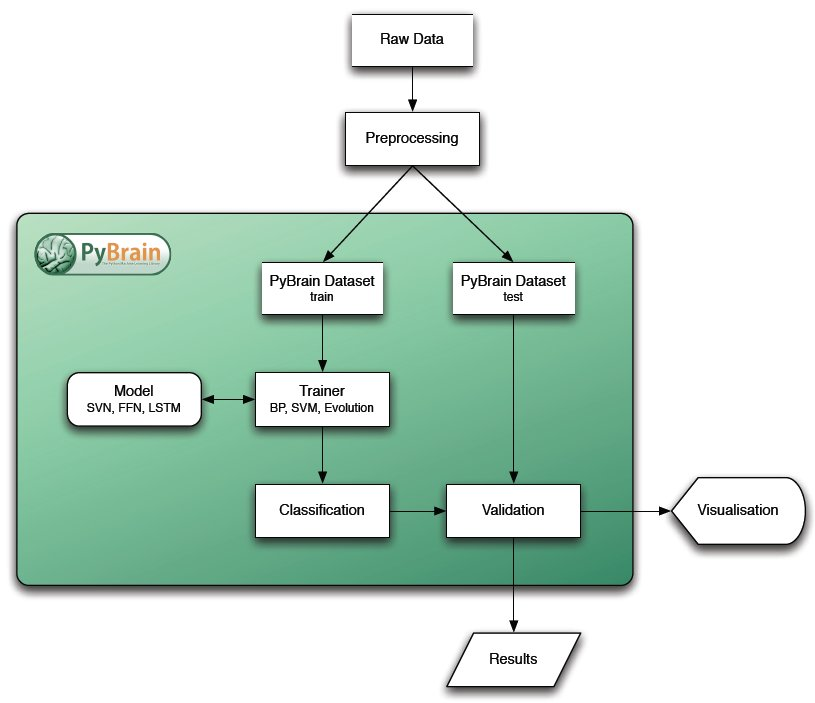
\includegraphics[width=0.7\linewidth]{figs/mlworkflow.jpg}
	\end{center}
\end{frame}

\subsection{Training and validation data sets}
\begin{frame}{Model validation}{Training and validation data sets}
	\small{
    	\begin{block}{}
       \vspace{-0.2cm}
       \lstinputlisting{code/dataset.py}
       \vspace{-0.2cm}
    	\end{block}
		}
\end{frame}

\section{Study case}
\begin{frame}{Study case}{Face recognition (I)}
   \begin{columns}
 	   \column{.50\textwidth}
	   The dataset:
	   \begin{itemize}
	   \item 40 people
	   \item 10 images for each person
	   \item 64x64 pixels
	   \item 40 x 10 = 400 samples
	   \end{itemize}
	\small \href{http://corpocrat.com/2014/10/10/tutorial-pybrain-neural-network-for-classifying-olivetti-faces/}{(Source)}
 	   \column{.50\textwidth}
		\begin{center}
		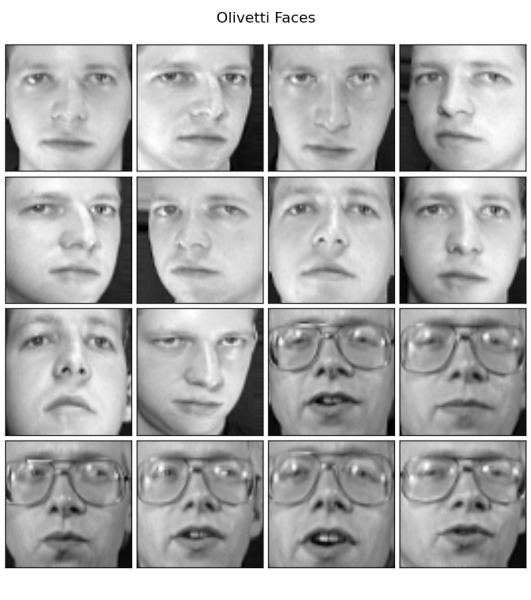
\includegraphics[width=0.9\linewidth]{figs/faces.png}
		\end{center}
	\end{columns}
\end{frame}

\begin{frame}{Study case}{Face recognition (II)}
   \begin{columns}
 	   \column{.50\textwidth}
	   The solution:
	   \begin{itemize}
	   \item Multilayer perceptron
	   \item Input layer: 64 x 64 = 4096 neurons
	   \item Hidden layer: 64 neurons, sigmoid
	   \item Output layer: 10 neurons, softmax
	   \item 40 x 10 = 400 samples
	   \end{itemize}
 	   \column{.50\textwidth}
		\begin{center}
		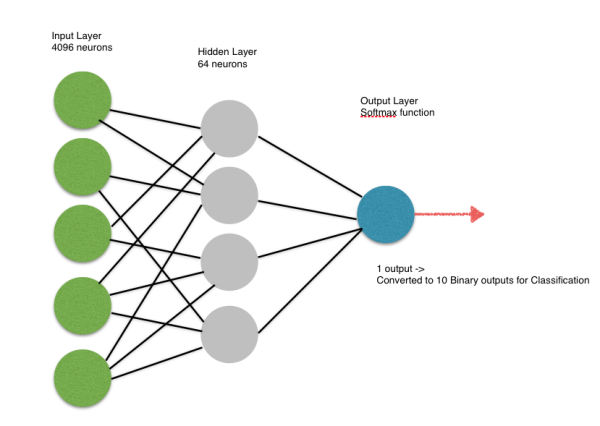
\includegraphics[width=\linewidth]{figs/nn.png}
		\end{center}
	\end{columns}
\end{frame}

\begin{frame}[plain, shrink]{Study case}{Face recognition (III)}
	\scriptsize{
    	\begin{block}{}
       \vspace{-0.2cm}
       \lstinputlisting{code/faces.py}
       \vspace{-0.2cm}
    	\end{block}
		}
\end{frame}

\section{Exercises}
\subsection{Introductory exercises}
\begin{frame}{Exercises}{Introductory exercises}
	Based on the template code given in the next slide, do the following tasks:
	\begin{enumerate}
		\item Substitute X by the proper values to train and validate a single neuron network with AND
			\begin{itemize}
			\item Which is the effect of parameters \texttt{learningrate} and \texttt{epochs}?
			\end{itemize}
		\item Train and validate a two neurons network with XOR
			\begin{itemize}
			\item Visualize weights (search the solution in Internet)
			\end{itemize}
		\item Train and validate a single neuron network with XOR
			\begin{itemize}
			\item What is happening?
			\end{itemize}
		\item Train and validate a 10 neuron network with XOR
			\begin{itemize}
			\item Use a \texttt{SoftmaxLayer} output layer. Analyze the result
			\end{itemize}
		\item Train and validate a 20 neuron network with XOR
			\begin{itemize}
			\item Increasing the network size improves the result?
			\end{itemize}
	\end{enumerate}
\end{frame}

\begin{frame}[plain, shrink]{Exercises}{Introductory exercises (II)}
	\scriptsize{
    	\begin{block}{}
       \vspace{-0.2cm}
       \lstinputlisting{code/ejercicio.py}
       \vspace{-0.2cm}
    	\end{block}
		}
\end{frame}

\subsection{Handwritting character recognition}
\begin{frame}{Exercises}{Handwritting character recognition (I)}
   \begin{columns}
 	   \column{.50\textwidth}
	Handwritting recognition
	\begin{enumerate}
		\item Download the dataset (\texttt{ex3data1.mat}) from \url{https://github.com/dfbarrero/aiCourse/tree/master/pybrain/datasets}
		\item Load dataset using the code shown in the next slide
		\item Complete the code to train and validate the neural network
	\end{enumerate}
 	   \column{.50\textwidth}
		\begin{center}
		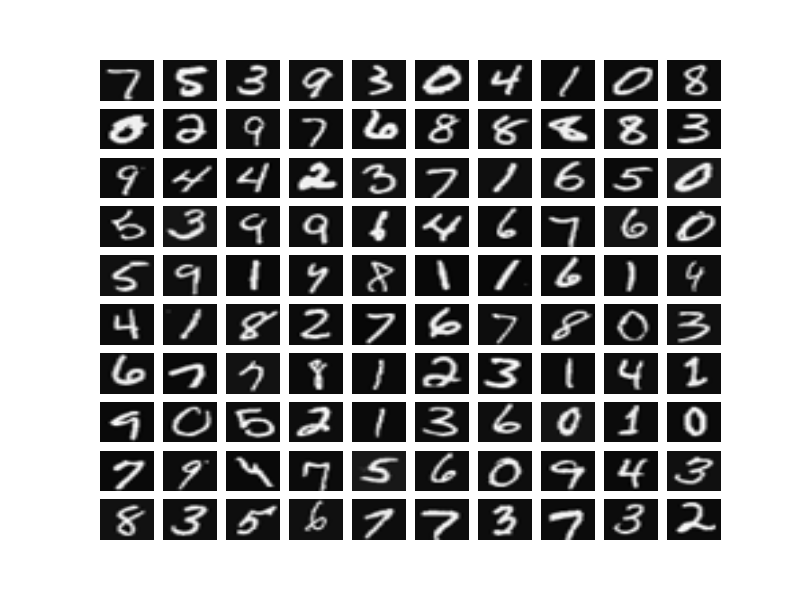
\includegraphics[width=\linewidth]{figs/hand.png}\\
	    \href{http://sujitpal.blogspot.com.es/2014/07/handwritten-digit-recognition-with.html}{(Source)}
		\end{center}
		\end{columns}
\end{frame}

\begin{frame}{Exercises}{Handwritting character recognition (II)}
    	\begin{block}{}
       \vspace{-0.2cm}
       \lstinputlisting{code/ejercicio2.py}
       \vspace{-0.2cm}
    	\end{block}
\end{frame}

\subsection{ANN integration with ROS}
\begin{frame}{Exercises}{ANN integration with ROS (I)}
	\begin{columns}
 	   \column{.70\textwidth}
	\begin{enumerate}
		\item Install Hector quadrotor: 
			\begin{itemize}
			\item \texttt{sudo apt-get install ros-indigo-hector-*}
			%\item \texttt{sudo apt-get install ros-indigo-hector-quadrotor-gazebo}
			\item Close the terminal and open a new one
			\end{itemize}
		\item Run simulation
			\begin{itemize}
			\item \texttt{roslaunch hector\_quadrotor\_demo outdoor\_flight\_gazebo.launch}
			\end{itemize}
		\item Run teleoperation (with joystick)
			\begin{itemize}
			\item \texttt{roslaunch hector\_quadrotor\_teleop xbox\_controller.launch}
			\end{itemize}
	\end{enumerate}
 	   \column{.30\textwidth}
		\centering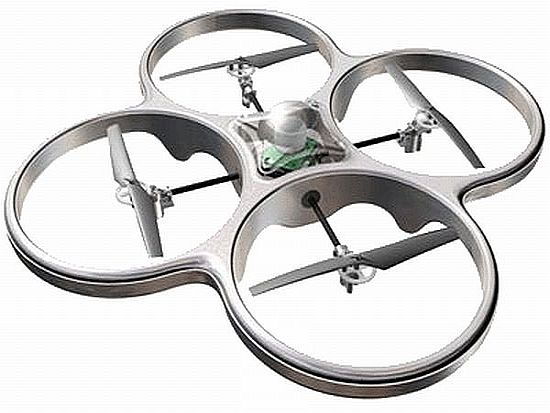
\includegraphics[width=\linewidth]{figs/quad.jpg}
	\end{columns}
\end{frame}

\begin{frame}{Exercises}{ANN integration with ROS (II)}
	Implement a \textbf{simple} altitude control in a UAV to keep it at $1.5\pm0.5 m$ over the ground
	\begin{enumerate}
		\item Locate the topic where sonar and an altimeter publish their data
		\item Identify which message types use the sonar and altimeter
		\item Locate the topic that controls the UAV motion
		\item Identify which message type is used to control the UAV motion
		\item Implement a node for altitude control
	\end{enumerate}
\end{frame}

\begin{frame}{Exercises}{ANN integration with ROS (III)}
	Implement a \textbf{neural} altitude control in a UAV to keep it at $1.5\pm0.5 m$ over the ground
	\begin{enumerate}
		\item Implement a node that capture data from the sonar and altimeter
		\item Build a dataset with the captured data, formatting and labeling it
			\begin{itemize}
			\item Hint: Use stdout redirection
			\end{itemize}
		\item Train an ANN with the layout that you prefere
		\item Validate the ANN
			\begin{itemize}
			\item Hint: Write a script that loads a network, reads the input form the keyboard and gives the ANN output
			\end{itemize}
		\item Integrate it in a ROS node
		\item Test the result
	\end{enumerate}
\end{frame}



\end{document}
